%% vim:tw=66:spell:wrap:ft=tex
\documentclass[%
        hyperref={%
                pdfauthor={Zakariyya Mughal},%
                pdfpagemode={None},pdfpagelayout={SinglePage}}%
        xcolor={x11names},%
]{beamer}
\usetheme{Warsaw}
\usecolortheme{crane}
\usepackage{textcomp}
\usepackage{fancyvrb}
\usepackage{changepage}
\usepackage{multicol}
\usepackage{wasysym}
\newenvironment{indented}{\begin{adjustwidth}{1.5em}{}}{\end{adjustwidth}}

\title[Vi/Vim]{Vi/Vim: Classic editors that can pack a punch}
\author{Zaki Mughal}
\institute{University of Houston:\\CougarCS}
\date{2010 Sept 02}
\begin{document}
\frame{\titlepage}


\begin{frame}
\frametitle{Pronunciation}
\begin{center}
\Huge
vi : /V.I./, not /vi/
\end{center}
\end{frame}

\begin{frame}
\frametitle{How to learn vi productively}
\begin{itemize}
\pause \item DRY: \emph{D}on't \emph{R}epeat \emph{Y}ourself
\pause \item premature optimization --- ``the root of all evil'':
\pause \par\begin{indented}learn as you go\end{indented}
\end{itemize}
\end{frame}

\begin{frame}[fragile]
\frametitle{Why}
\begin{itemize}
\pause \item classic Unix editor --- part of the POSIX standard
\pause \item available on most Unix systems
\pause \item efficient editing for text typists\ldots, e.g.
	\begin{itemize}
	\item \Verb+ddp+ --- swap lines
	\item \Verb+xp+ --- swap letters
	\end{itemize}
\pause \item large files open \emph{quickly}
\end{itemize}
\end{frame}

\begin{frame}
\frametitle{Why not}
\begin{itemize}
\item unintuitive
\item addictive
\item puzzling for others
\pause
\item your mouse will feel lonely
\end{itemize}
\end{frame}

\begin{frame}
\frametitle{History}
\begin{itemize}
\item Bill Joy @ UC Berkeley in 1976
\item \Verb+ed+itor $\Rightarrow$ \Verb+ex+tended $\Rightarrow$
\Verb+vi+sual
\item clones: Vim
\end{itemize}
\end{frame}

\begin{frame}
\frametitle{Modal interface}
\begin{itemize}
\item normal mode
\item command-line mode
\item insert mode
\end{itemize}
\pause
\begin{beamerboxesrounded}{Tip}
Always use the \Verb+Escape+ key (alternatively \Verb+Control-[+).
In Vim, show commands at the bottom of the screen using \Verb+:set showcmd+
\end{beamerboxesrounded}
\end{frame}

\begin{frame}[fragile]
\frametitle{Handling files}
\begin{itemize}
\item from the command line
	\begin{indented}
	\begin{Verbatim}
	vi [filename]
	\end{Verbatim}
	\end{indented}
\pause \item quitting
	\begin{itemize}
	\item \Verb+:q+
	\item \Verb+:q!+ or \Verb+ZQ+
	\end{itemize}
\pause \item saving
	\begin{itemize}
	\item \Verb+:w [filename]+
	\item \Verb+:w+
	\item \Verb+:wq+ and \Verb+:wq!+ or ZZ
	\item force overwrite: \Verb+:w!+
	\end{itemize}
\pause \item opening files
	\begin{itemize}
	\item \Verb+:e [filename]+
	\end{itemize}
\end{itemize}
\end{frame}

\begin{frame}
\frametitle{Appeasing vi enough to actually take input}
\begin{itemize}
\item Enter insert mode
\item Before the cursor: \Verb+i+
\item After the cursor: \Verb+a+
\item \Verb+I+, \Verb+A+
\end{itemize}
\end{frame}

\begin{frame}[allowframebreaks]
\frametitle{Navigating a file}
\begin{center}
\Huge
$\overset{\leftarrow}{\text{h}}\qquad
\overset{\downarrow}{\text{j}}\qquad
\overset{\uparrow}{\text{k}}\qquad
\overset{\rightarrow}{\text{l}}$
\end{center}
\framebreak
\begin{figure}
\framebox{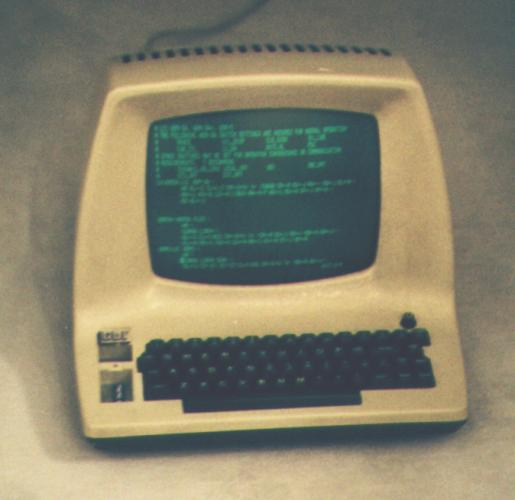
\includegraphics[width=0.6\textwidth]{gfx/adm3a-4.jpg}}
\caption{ADM-3A terminal {\tiny [Source:
\url{http://www.tentacle.franken.de/adm3a/adm3a-4.html}]
} }
\end{figure}
\framebreak
\begin{figure}
\framebox{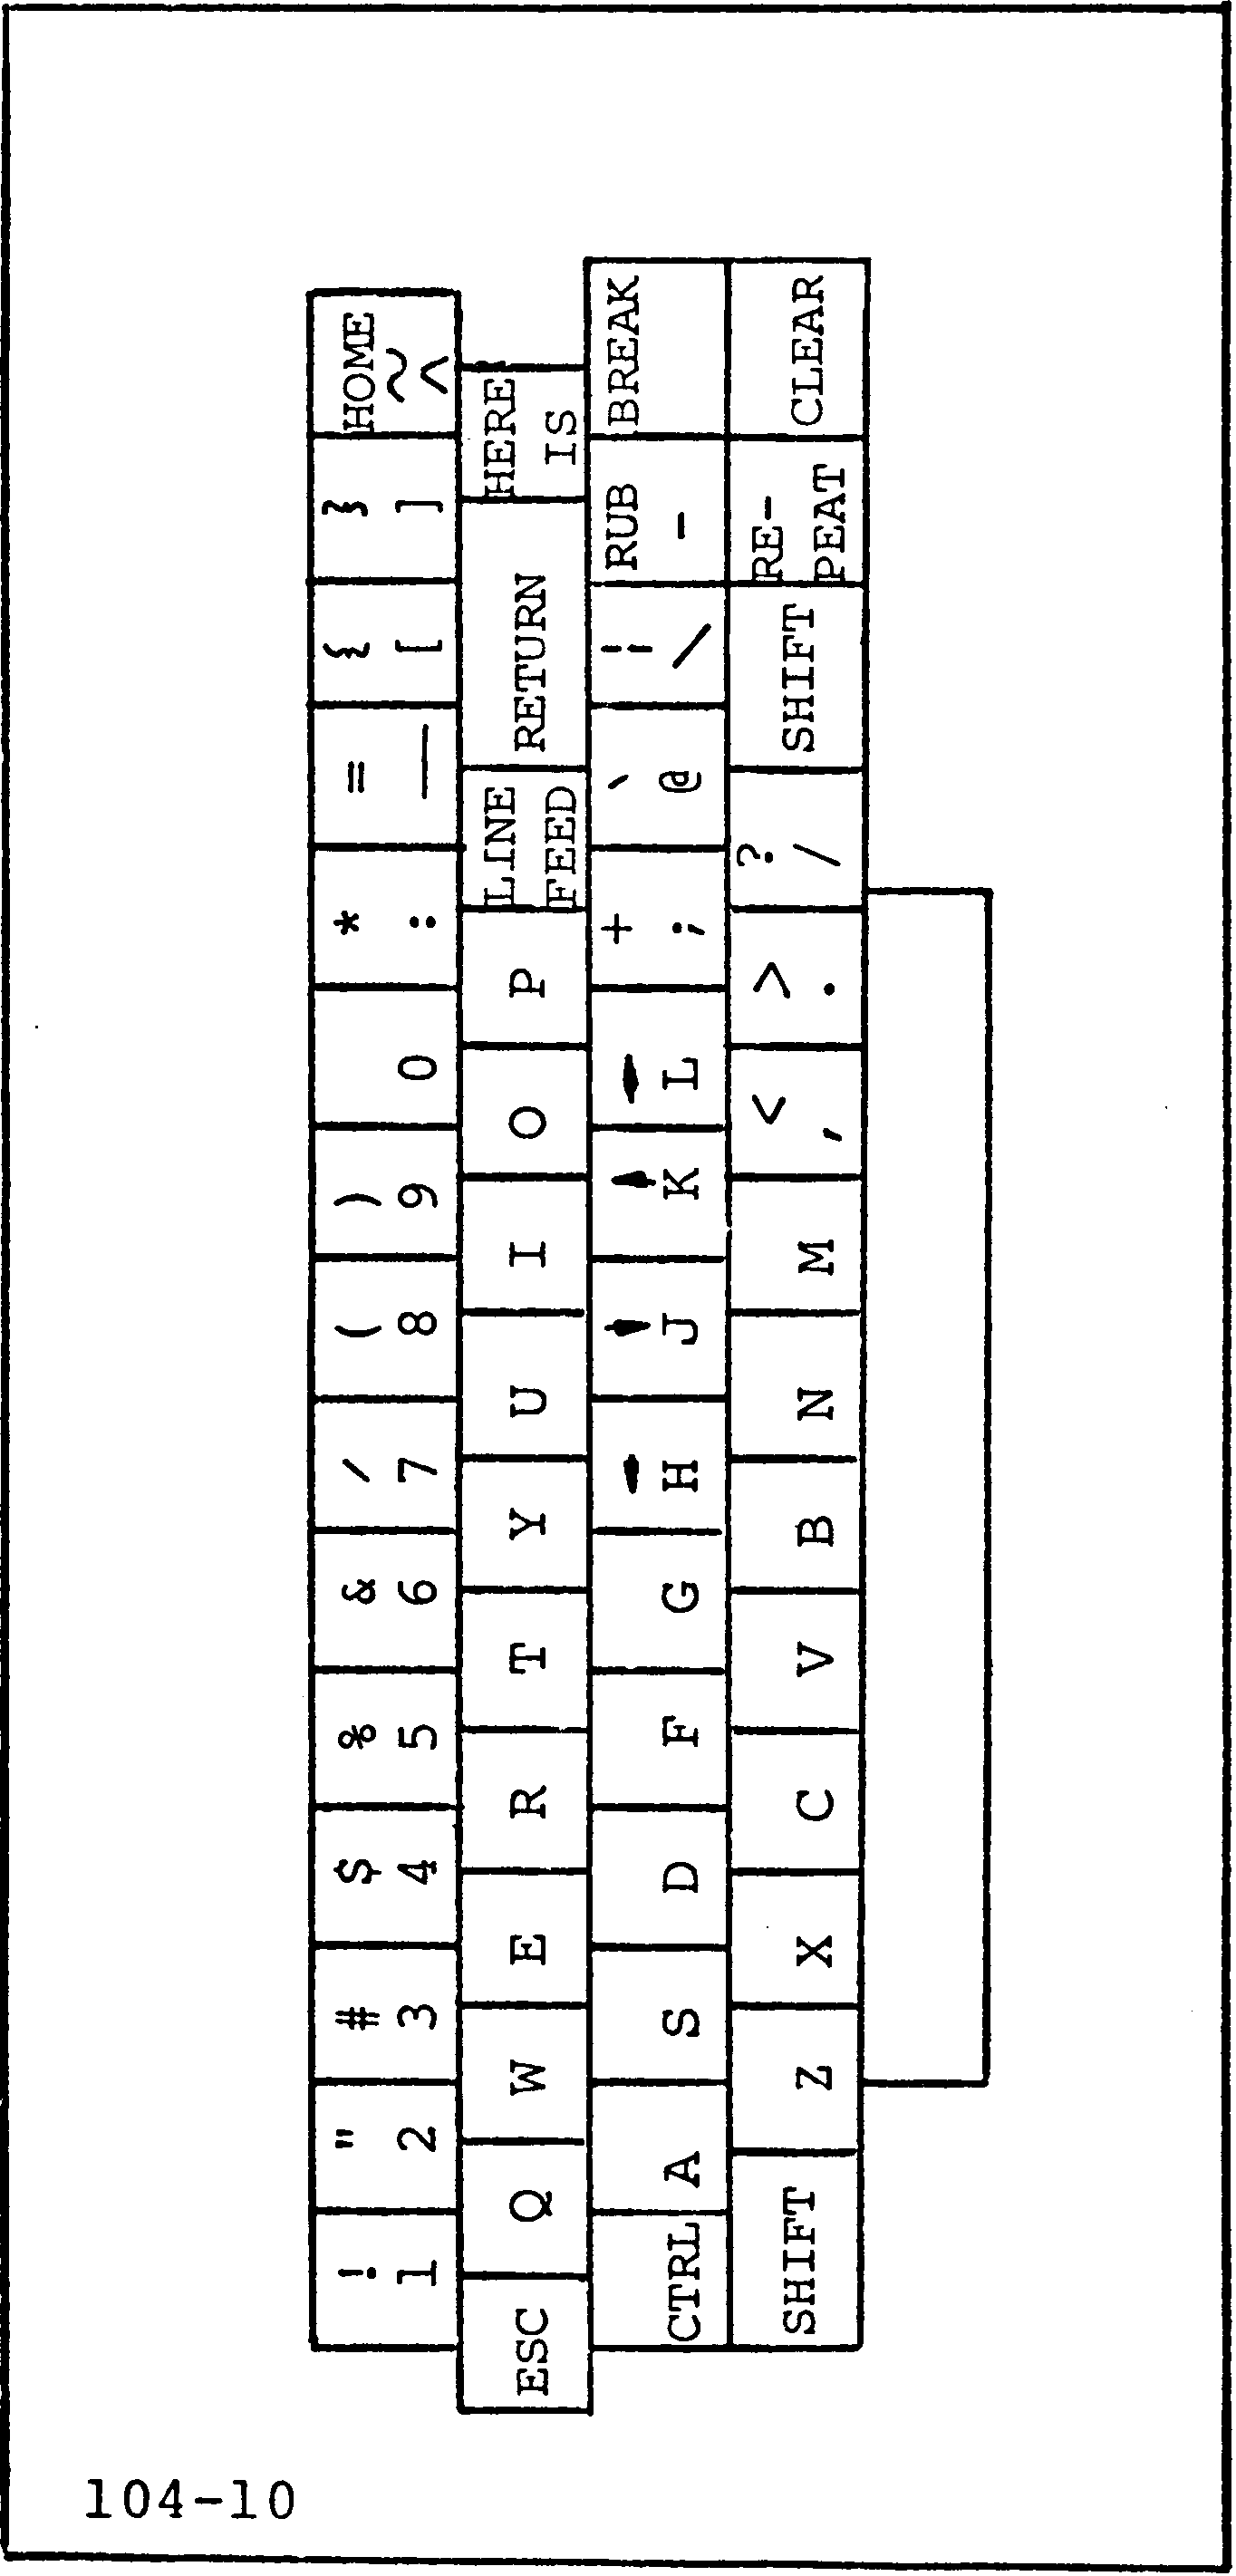
\includegraphics[angle=-90,width=0.95\textwidth]{gfx/adm3a-kbd.png}}
\caption{ADM-3A keyboard {\tiny [Source:
\url{http://vt100.net/lsi/adm3a-om/}, pg. 36]
} }
\end{figure}
\framebreak
\begin{itemize}
\item Skipping words: \Verb+w+, \Verb+e+, \Verb+b+
\item Search
\begin{itemize}
\item \Verb+/+ : forwards; \Verb+?+ : backwards
\item [Vim] \Verb+set incsearch hlsearch+
\item \Verb+n+, \Verb+N+
\item \Verb+*+, \Verb+\#+
\end{itemize}
\item \Verb+gg+, \Verb+G+ ; take a count before the command
\item \Verb+H+, \Verb+L+, \Verb+M+
\item Sentences: \Verb+(+, \Verb+)+
\item Paragraphs: \Verb+\{+, \Verb+\}+
\item Matching pair of braces: \Verb+\%+
\item Ends of line: \Verb+0+, \texttt{\^}, \Verb+\$+ % TODO: circumflex
\item Jump to characters: \Verb+f+, \Verb+F+, \Verb+t+, \Verb+T+,
\Verb+;+ \Verb+,+
\end{itemize}
\end{frame}

\begin{frame}
\frametitle{Wait, I need to change something}
\begin{itemize}
\item in insert mode: \Verb+Control-W+, \Verb+Control-U+, \Verb+Delete+,
\Verb+Backspace+
\item \Verb+r+, \Verb+R+
\item \Verb+x+, \Verb+X+
\item \Verb+d+ + motion; [Vim]: text objects
\item \Verb+D+, \Verb+dd+
\item \Verb+c+
\item \Verb+S+
\item [Vim]: \Verb+gu+ + motion , \Verb+gU+ + motion
\end{itemize}
\end{frame}

\begin{frame}
\frametitle{Copy and pasta}
\begin{itemize}
\item \Verb+y+ + motion
\item \Verb+yy+
\item \Verb+p+, \Verb+P+
\item registers
\item in insert mode: \Verb+Control-E+, \Verb+Control-Y+
\end{itemize}
\end{frame}

\begin{frame}
\frametitle{Visual mode [Vim]}
\begin{itemize}
\item \Verb+v+
\item linewise: \Verb+V+
\item blockwise: \Verb+Control-V+
\end{itemize}
\end{frame}


\begin{frame}
\frametitle{The edit, compile, run cycle [Vim]}
\begin{itemize}
\item \Verb+:set makeprg+, \Verb+:compiler+, \Verb+:copen+,
\Verb+:cnext+, \Verb+:cNext+
\item \Verb+:set grepprg+, \Verb+:grep+
\end{itemize}
\end{frame}

\begin{frame}[fragile]
\frametitle{Vi has a couple more tricks up its sleeve}
\begin{itemize}
\item filter through pipe: \Verb+\%![exec]+
\item maps
	\begin{indented}
	\begin{Verbatim}
	:nmap ,tw	:set wrap!<CR>
	\end{Verbatim}
	\end{indented}
\item abbreviations
	\begin{indented}
	\begin{Verbatim}
	:abbr teh the
	\end{Verbatim}
	\end{indented}
\item marks
\end{itemize}
\end{frame}

\begin{frame}
\frametitle{More complex changes}
\begin{itemize}
\item repeat: \Verb+.+
\item \Verb+:substitute+
\item \Verb+:global+
\end{itemize}
\end{frame}

\begin{frame}
\frametitle{\ldots{}and Vim has many, many more}
\begin{multicols}{2}
\begin{itemize}
\item scriptable
\item swap files
\item syntax highlighting
\item extended regexps
\item folds
\item programmable indentation
\item formatting
\item directory viewer
\item (S)FTP/HTTP/WebDAV
\item compressed archives and files
\item multi-level undo with branching
\item split windows
\item tabs
\item \Verb+ctags+
\item spell checking
\item programmable completion
\item jumps
\item \Verb+gf+, \Verb+Control-W gf+
\item Plugins
\begin{itemize}
\item NERDTree, NERDCommenter
\item Taglist
\item BufExplorer, FuzzyFinder
\item A.vim, Align, Matchit
\item surround
\item Matrix
\end{itemize}
\end{itemize}
\end{multicols}
\end{frame}

\begin{frame}[fragile]
\frametitle{Resources}
\begin{itemize}
\item \Verb+vimtutor+
\item online \Verb+:help+
\begin{indented}
\begin{Verbatim}
:help <Control-D>
:help <Tab>
:helpgrep [regexp]
\end{Verbatim}
\end{indented}
\item The Internet
\item \href{http://www.vi-improved.org/}{\Verb+\#vim+ IRC channel on Freenode}
\item \href{http://groups.google.com/group/vim_use}{\Verb+vim\_use+ mailing list}
\item \href{http://vim.wikia.com/wiki/Vim_Tips_Wiki}{Vim Tips Wikia}
\item \href{http://www.viemu.com/a_vi_vim_graphical_cheat_sheet_tutorial.html}{Cheatsheet from ViEmu}
\pause \item Me \smiley
\end{itemize}
\end{frame}

\begin{frame}
\frametitle{\textinterrobang}
\begin{center}
\Huge
Questions?\\Complaints!
\end{center}
\end{frame}

\end{document}
